\documentclass[a4paper,11pt]{article} % This defines the style of your paper

\usepackage[top = 1in, bottom = 0.8in, left = 0.5in, right = 0.5in]{geometry}
\usepackage{float}
\usepackage{fancyhdr}
\usepackage{setspace}
\setlength{\parindent}{0in}
\usepackage{tikz-qtree}

\usepackage{listings}
\usepackage{color}

\definecolor{dark_green}{rgb}{0,0.6,0}
\definecolor{gray}{rgb}{0.5,0.5,0.5}
\definecolor{mauve}{rgb}{0.58,0,0.82}

\lstset{
  frame=none,
  language=C,
  columns=flexible,
  basicstyle={\small\ttfamily},
  numbers=none,
  numberstyle=\tiny\color{gray},
  keywordstyle=\color{blue},
  commentstyle=\color{dark_green},
  stringstyle=\color{mauve},
  breakatwhitespace=true,
  tabsize=2
}

\usepackage{graphicx}

\newcommand{\code}[1]{\texttt{#1}}

\pagestyle{fancy}
\fancyhf{}

\lhead{\footnotesize Programming Languages Homework 1}
\rhead{\footnotesize Peng-Yu Chen}
\cfoot{\footnotesize \thepage}

\begin{document}
\thispagestyle{empty}

\begin{tabular}{p\linewidth}
{\large \bf Programming Languages - Homework 1} \\ Name: Peng-Yu Chen (pyc305) \\
\hline
\end{tabular}

\vspace{0.4cm}

\begin{enumerate}
  \item % 1.
  \begin{enumerate}
    \item \code{[a-z]*[A-Z][a-z]*[0-9][a-z]*[A-Z][a-z]*}
    \item \code{(-|+|$\epsilon$)[0-9][0-9]*.[0-9][0-9]*E(-|+|$\epsilon$)[0-9][0-9]*}
    \item \code{[a-zA-Z]([a-zA-Z0-9\_]|$\epsilon$)([a-zA-Z0-9\_]|$\epsilon$)
      ([a-zA-Z0-9\_]|$\epsilon$)([a-zA-Z0-9\_]|$\epsilon$) \\
      ([a-zA-Z0-9\_]|$\epsilon$)([a-zA-Z0-9\_]|$\epsilon$)}
  \end{enumerate}

  \item % 2.
  \begin{enumerate}
    \item % (a)
    \code{PROG $\to$ DECLS} \\
    \code{DECLS $\to$ DECL DECLS | DECL} \\
    \code{DECL $\to$ VARDECL ; | FUNDECL | PROCDECL} \\

    \code{VARDECL $\to$ ID : int} \\
    \code{FUNDECL $\to$ fun SIGNATURE } \\
    \code{PROCDECL $\to$ proc SIGNATURE } \\
    \code{SIGNATURE $\to$ ID ( PARAMLIST ) DECLS BLOCK } \\

    \code{PARAMLIST $\to$ PARAMS | $\epsilon$} \\
    \code{PARAMS $\to$ VARDECL | VARDECL , PARAMS} \\
    \code{BLOCK $\to$ \{ STMTS \}} \\

    \code{STMTS $\to$ STMT STMTS | STMT} \\
    \code{STMT $\to$ ASMT | RETURN} \\
    \code{ASMT $\to$ ID = E ;} \\
    \code{RETURN $\to$ return E ;} \\

    \code{E $\to$ T | T + T} \\
    \code{T $\to$ F | F - F} \\
    \code{F $\to$ ID | NUM | FUNCALL} \\

    \code{FUNCALL $\to$ ID ( ARGLIST )} \\
    \code{ARGLIST $\to$ ARGS | $\epsilon$} \\
    \code{ARGS $\to$ E | E, ARGS}

    \item % (b)
    \phantom{}

    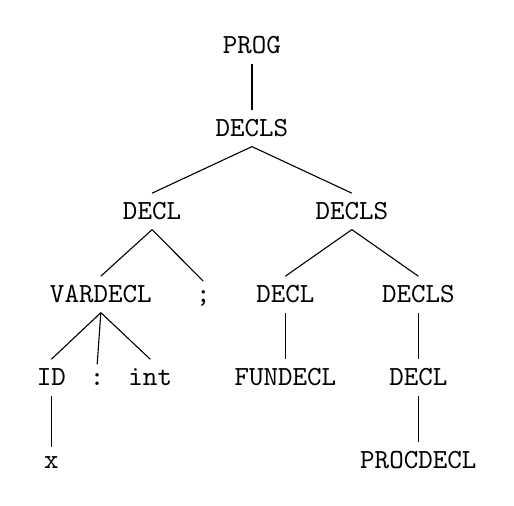
\begin{tikzpicture}[scale=1.0]
    \Tree [.\code{PROG} [.\code{DECLS}
      [.\code{DECL}
        [.\code{VARDECL}
          [.\code{ID} [.\code{x} ]]
          [.\code{:} ]
          [.\code{int} ]
        ]
        [.\code{;} ]
      ]
      [.\code{DECLS}
        [.\code{DECL} [.\code{FUNDECL} ]]
        [.\code{DECLS} [.\code{DECL} [.\code{PROCDECL} ]]]
      ]
    ]]
    \end{tikzpicture}

    (see next page for detailed \code{FUNDECL} and \code{PROCDECL})

    \newpage

    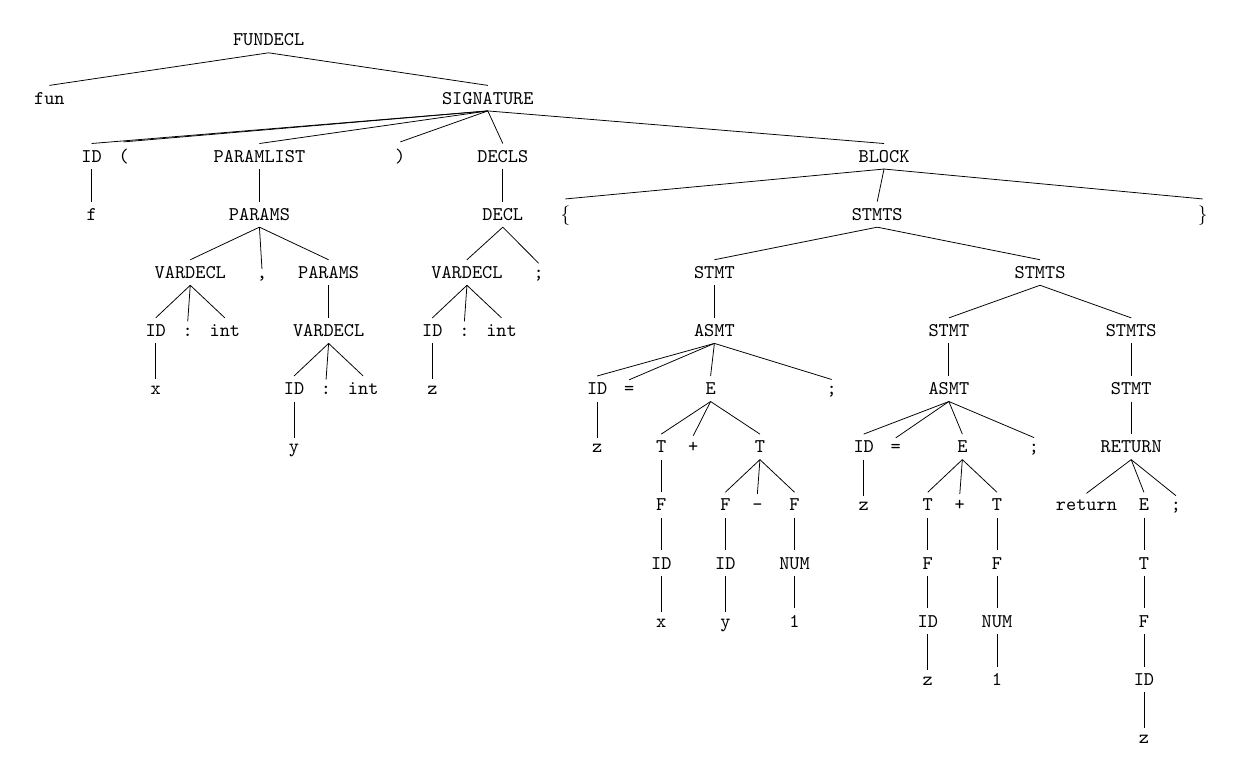
\begin{tikzpicture}[scale=0.7]
    \Tree [.\code{FUNDECL}
      [.\code{fun} ]
      [.\code{SIGNATURE}
        [.\code{ID} [.\code{f} ]]
        [.\code{(} ]
        [.\code{PARAMLIST}
          [.\code{PARAMS}
            [.\code{VARDECL}
              [.\code{ID} [.\code{x} ]]
              [.\code{:} ]
              [.\code{int} ]
            ]
            [.\code{,} ]
            [.\code{PARAMS}
              [.\code{VARDECL}
                [.\code{ID} [.\code{y} ]]
                [.\code{:} ]
                [.\code{int} ]
              ]
            ]
          ]
        ]
        [.\code{)} ]
        [.\code{DECLS}
          [.\code{DECL}
            [.\code{VARDECL}
              [.\code{ID} [.\code{z} ]]
              [.\code{:} ]
              [.\code{int} ]
            ]
            [.\code{;} ]
          ]
        ]
        [.\code{BLOCK}
          [.\code{\{} ]
          [.\code{STMTS}
            [.\code{STMT}
              [.\code{ASMT}
                [.\code{ID} [.\code{z} ]]
                [.\code{=} ]
                [.\code{E}
                  [.\code{T} [.\code{F} [.\code{ID} [.\code{x} ]]]]
                  [.\code{+} ]
                  [.\code{T}
                    [.\code{F} [.\code{ID} [.\code{y} ]]]
                    [.\code{-} ]
                    [.\code{F} [.\code{NUM} [.\code{1} ]]]
                  ]
                ]
                [.\code{;} ]
              ]
            ]
            [.\code{STMTS}
              [.\code{STMT}
                [.\code{ASMT}
                  [.\code{ID} [.\code{z} ]]
                  [.\code{=} ]
                  [.\code{E}
                    [.\code{T} [.\code{F} [.\code{ID} [.\code{z} ]]]]
                    [.\code{+} ]
                    [.\code{T} [.\code{F} [.\code{NUM} [.\code{1} ]]]]
                  ]
                  [.\code{;} ]
                ]
              ]
              [.\code{STMTS}
                [.\code{STMT}
                  [.\code{RETURN}
                    [.\code{return} ]
                    [.\code{E} [.\code{T} [.\code{F} [.\code{ID} [.\code{z} ]]]]]
                    [.\code{;} ]
                  ]
                ]
              ]
            ]
          ]
          [.\code{\}} ]
        ]
      ]
    ]
    \end{tikzpicture}

    \begin{tikzpicture}[scale=0.7]
    \Tree [.\code{PROCDECL}
      [.\code{proc} ]
      [.\code{SIGNATURE}
        [.\code{ID} [.\code{g} ]]
        [.\code{(} ]
        [.\code{PARAMSLIST} [.\code{$\epsilon$} ]]
        [.\code{)} ]
        [.\code{DECLS}
          [.\code{DECL}
            [.\code{VARDECL}
              [.\code{ID} [.\code{a} ]]
              [.\code{:} ]
              [.\code{int} ]
            ]
            [.\code{;} ]
          ]
        ]
        [.\code{BLOCK}
          [.\code{\{} ]
          [.\code{STMTS}
            [.\code{STMT}
              [.\code{ASMT}
                [.\code{ID} [.\code{a} ]]
                [.\code{=} ]
                [.\code{E} [.\code{T} [.\code{F} [.\code{NUM} [.\code{3} ]]]]]
                [.\code{;} ]
              ]
            ]
            [.\code{STMTS}
              [.\code{STMT}
                [.\code{ASMT}
                  [.\code{ID} [.\code{x} ]]
                  [.\code{=} ]
                  [.\code{E} [.\code{T} [.\code{F} [.\code{FUNCALL}
                    [.\code{ID} [.\code{f} ]]
                    [.\code{(} ]
                    [.\code{ARGLIST}
                      [.\code{ARGS}
                        [.\code{E} [.\code{T} [.\code{F} [.\code{ID} [.\code{a} ]]]]]
                        [.\code{,} ]
                        [.\code{ARGS} [.\code{E} [.\code{T} [.\code{F} [.\code{NUM} [.\code{2} ]]]]]]
                      ]
                    ]
                    [.\code{)} ]
                  ]]]]
                  [.\code{;} ]
                ]
              ]
            ]
          ]
          [.\code{\}} ]
        ]
      ]
    ]
    \end{tikzpicture}
  \end{enumerate}

  \item % 3.

  \begin{enumerate}
    \item % (a)
    \begin{itemize}
      \item \textit{static scoping}: the scope of a variable is evaluated in the
      environment of where it's defined.
      \item \textit{dynamic scoping}: the scope of a variable is evaluated in the
      environment of where it's called.
    \end{itemize}

\newpage

    \item % (b)
\begin{lstlisting}
  void A() {
    int x;    // static scoping will update this x

    void B() {
      x = 1;
    }

    void C() {
      int x;  // dynamic scoping will update this x
      B();
    }

    C();
  }
\end{lstlisting}

    \item % (c)
    \begin{itemize}
      \item Compile-time: to find the declaration of a variable in a statically
      scoped language, if we can find the declaration locally, then we use it;
      otherwise, it is a non-local variable, so we have to look at the scope in
      the same level of the definition of the function/procedure.
      \item Run time: we can find the reference of a variable by traversing the
      static link for pre-computed jumps in languages that support nested procedures.
    \end{itemize}

    \item % (d)
    To find the declaration of a variable in a dynamically scoped language,
    if we can find the declaration locally, then we use it; otherwise, is a
    non-local variable so we have to look at the scope in the same level of the
    calling of the function/procedure by traversing the dynamic link and
    checking each stack frame until we find the variable.

  \end{enumerate}

  \item % 4
  \phantom{}

  \begin{minipage}[t]{\linewidth}
    \begin{center}
      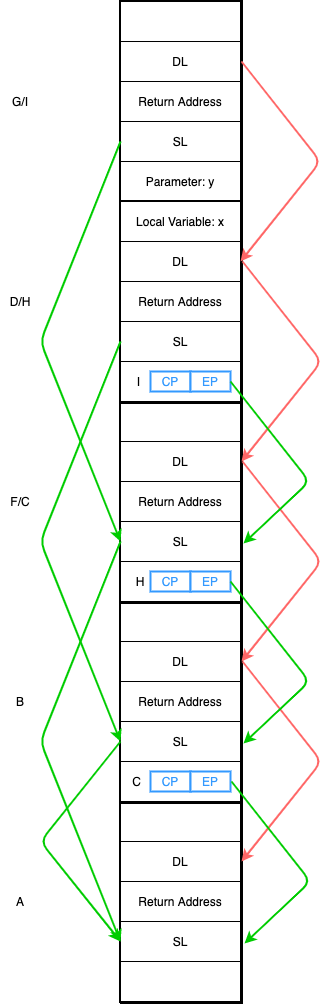
\includegraphics[width=0.25\linewidth]{./images/4.png}
    \end{center}
  \end{minipage}

  \item % 5
  \begin{enumerate}
    \item \code{2 4 6 8 10}
    \item \code{2 11 6 8 10}
    \item \code{2 7 6 8 10}
    \item \code{2 4 6 8 11}
  \end{enumerate}

  \item % 6
  \begin{enumerate}
    \item % (a)
\begin{lstlisting}
  with Ada.Text_IO;
  use Ada.Text_IO;

  procedure Print_Numbers is
    package Int_IO is new Ada.Text_IO.Integer_IO(Integer);
    use Int_IO;

    task T1 is
      entry Start;
    end T1;

    task T2 is
      entry Start;
    end T2;

    task body T1 is
    begin
      for I in 1..100 loop
        Put(I);
        if I mod 10 = 0 then
          T2.Start;
          accept Start;
        end if;
      end loop;
    end T1;

    task body T2 is
    begin
      for I in 201..300 loop
        if I mod 10 = 1 then
          accept Start;
        end if;
        Put(I);
        if I mod 10 = 0 then
          T1.Start;
        end if;
      end loop;
    end T2;

  begin
    null;
  end Print_Numbers;
\end{lstlisting}
    \item % (b)
    No, the printing of the numbers is not occurring concurrently.
    The order in which numbers should be printed is already determined,
    while concurrency means that we don't know which event will occur first.

  \end{enumerate}

\end{enumerate}

\end{document}
